\documentclass{article}

% We suggest
% if you need to pass options to natbib, use, e.g.:
%     \PassOptionsToPackage{numbers, compress}{natbib}
% before loading neurips_2020

% ready for submission
% \usepackage{neurips_2020}

% to compile a preprint version, e.g., for submission to arXiv, add add the
% [preprint] option:
%     \usepackage[preprint]{neurips_2020_tda}

% to compile a camera-ready version, add the [final] option, e.g.:
\usepackage[final,nonatbib]{neurips_2020_tda}

% to avoid loading the natbib package, add option nonatbib:
%\usepackage[nonatbib]{neurips_2020_tda}

\usepackage[utf8]{inputenc} % allow utf-8 input
\usepackage[T1]{fontenc}    % use 8-bit T1 fonts
\usepackage{amsfonts}       % blackboard math symbols
\usepackage{booktabs}       % professional-quality tables
\usepackage{hyperref}       % hyperlinks
\usepackage{url}            % simple URL typesetting
\usepackage{microtype}      % microtypography
\usepackage{nicefrac}       % compact symbols for 1/2, etc.
\usepackage{paralist}       % in-paragraph enumerations
\usepackage{siunitx}        % SI units


\usepackage{subcaption}


\usepackage{amsmath,amssymb,amsfonts,amsthm}
\usepackage{microtype}
%\usepackage[draft]{fixme}
\usepackage{algorithmic}
\usepackage{graphicx}
\usepackage{textcomp}
\usepackage{xcolor}
\usepackage{tikz}
\usepackage{mwe}

\newsavebox{\tempbox}
\newlength{\tempwidth}


\usepackage[natbib,hyperref,sorting=none]{biblatex}
%\usepackage[backend=bibtex,doi=true,style=numeric,maxnames=3,maxbibnames=6]{biblatex}
\addbibresource{bibliography.bib}
%\renewcommand*{\bibfont}{\footnotesize}

\urlstyle{same}

\title{
  Simplicial Neural Networks
}

% The \author macro works with any number of authors. There are two commands
% used to separate the names and addresses of multiple authors: \And and \AND.
%
% Using \And between authors leaves it to LaTeX to determine where to break the
% lines. Using \AND forces a line break at that point. So, if LaTeX puts 3 of 4
% authors names on the first line, and the last on the second line, try using
% \AND instead of \And before the third author name.

\author{%
  David S.~Hippocampus\thanks{Use footnote for providing further information
    about author (webpage, alternative address)---\emph{not} for acknowledging
    funding agencies.} \\
  Department of Computer Science\\
  Cranberry-Lemon University\\
  Pittsburgh, PA 15213 \\
  \texttt{hippo@cs.cranberry-lemon.edu} \\
  % examples of more authors
  % \And
  % Coauthor \\
  % Affiliation \\
  % Address \\
  % \texttt{email} \\
  % \AND
  % Coauthor \\
  % Affiliation \\
  % Address \\
  % \texttt{email} \\
  % \And
  % Coauthor \\
  % Affiliation \\
  % Address \\
  % \texttt{email} \\
  % \And
  % Coauthor \\
  % Affiliation \\
  % Address \\
  % \texttt{email} \\
}
\theoremstyle{definition}
\newtheorem{definition}{Definition}
\newtheorem{example}[definition]{Example}
\newtheorem{note}[definition]{Note}

\theoremstyle{plain}
\newtheorem{theorem}[definition]{Theorem}
\newtheorem{lemma}[definition]{Lemma}
\newtheorem{proposition}[definition]{Proposition}
\newtheorem{corollary}[definition]{Corollary}

\definecolor{mplC0}{HTML}{1f77b4}
\definecolor{mplC1}{HTML}{ff7f0e}
\definecolor{mplC2}{HTML}{2ca02c}
\definecolor{mplC3}{HTML}{d62728}
\definecolor{mplC4}{HTML}{9467bd}
\definecolor{mplC5}{HTML}{8c564b}
\definecolor{mplC6}{HTML}{e377c2}
\definecolor{mplC7}{HTML}{7f7f7f}
\definecolor{mplC8}{HTML}{bcbd22}
\definecolor{mplC9}{HTML}{17becf}

\newcommand{\RR}{\ensuremath{\mathbb{R}}}
\newcommand{\ZZ}{\ensuremath{\mathbb{Z}}}
\newcommand{\RP}{\ensuremath{\mathbb{RP}}}
\newcommand{\lapu}{\ensuremath{\mathcal{L}^{\text{up}}}}
\newcommand{\lapd}{\ensuremath{\mathcal{L}^{\text{down}}}}
\newcommand{\lap}{\ensuremath{\mathcal{L}}}
\newcommand{\iso}{\ensuremath{\cong}}
\newcommand{\rank}{\ensuremath{\text{rank}}}
\newcommand{\inv}{\ensuremath{^{-1}}}
\newcommand{\transpose}{\ensuremath{^{\intercal}}}

\tikzset{twosimp/.style={fill opacity=0.4,fill=blue,draw opacity=1.0}}

\newcommand{\ie}{}
\def\ie/{i.e.}
\newcommand{\eg}{}
\def\eg/{e.g.}
\newcommand{\etc}{}
\def\etc/{etc.}

\newcommand{\gardfix}[2]{{\color{red}#1}\fxfatal{#2}}
\newcommand{\fix}[2]{{\color{red}#1}\fxfatal{#2}}
\newcommand{\thmcite}[1]{\citeauthor{#1}, \citeyear{#1}~\cite{#1}}
\newcommand{\suchthat}{\ensuremath{\, \mid \,}}

\newcommand{\Reffig}[1]{Figure~\ref{fig:#1}}
\newcommand{\reffig}[1]{figure~\ref{fig:#1}}
\newcommand{\refeq}[1]{equation~\eqref{eq:#1}}
\newcommand{\refsec}[1]{section~\ref{sec:#1}}

\newcommand{\ip}[2]{\ensuremath{\left\langle #1 , #2 \right\rangle}}
\newcommand{\norm}[1]{\ensuremath{\lVert #1 \rVert}}

\newcommand{\placeholderfigure}{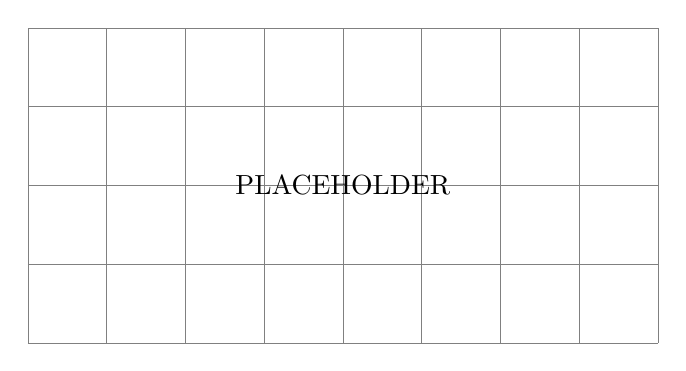
\begin{tikzpicture}
      \draw[help lines] (0, 0) grid (8, 4);
      \node () at (4,2) {PLACEHOLDER};
  \end{tikzpicture}
}

\DeclareMathOperator{\cut}{cut}
\DeclareMathOperator{\im}{im}
\DeclareMathOperator{\proj}{proj}
\DeclareMathOperator{\VR}{VR}
\DeclareMathOperator{\diag}{diag}


%---------For commenting--------
\usepackage{color}
\definecolor{darkorchid}{rgb}{0.6,0.196,0.8}
\newcommand{\todo}[1]{{\color{red}[[\textbf{TODO: }#1]]}}
\newcommand{\stefania}[1]{{\color{mplC0}[[\textbf{Stefania says: }#1]]}}
\newcommand{\gard}[1]{{\color{mplC2}[[\textbf{Gard says: }#1]]}}
\newcommand{\mdeff}[1]{{\color{mplC1}[[\textbf{Michaël says: }#1]]}}

%--------For Referencing--------
\newcommand{\appendref}[1]{Section~\ref{append:#1}}
\newcommand{\figref}[1]{Figure~\ref{fig:#1}}
\newcommand{\exref}[1]{Example~\ref{ex:#1}}
\newcommand{\secref}[1]{Section~\ref{sec:#1}}
\newcommand{\Thmref}[1]{Theorem~\ref{thm:#1}}
\newcommand{\thmref}[1]{Theorem~\ref{thm:#1}}
\newcommand{\defref}[1]{Definition~\ref{def:#1}}


\begin{document}

\maketitle

\begin{abstract}
In this paper we present simplicial neural networks (SNNs), a generalization of graph convolutional neural networks to data that live on a class of topological spaces called simplicial complexes. These are natural multi-dimensional extensions of graphs which encode more than just pairwise relationships, namely higher-order interactions between nodes (represented geometrically as filled triangles, tetrahedra, and so forth). We define an appropriate notion of convolutions for such data, which we leverage to construct the desired convolutional neural networks. This allows us to consider richer data than traditional methods, including vector field data and $n$-fold collaboration networks. Finally, we test the ability of the SNNs on the task of imputing missing data on simplicial complexes built from coauthorship data.
  
\end{abstract}


\section{Introduction}



Graph-based convolutional neural networks (GNNs) have recently become popular techniques in machine learning \stefania{cite}. Compared to classical deep neural networks dealing with regular grid-structured data, graph neural networks take into account irregular graphs to better learn complex interactions in the data. Although graphs can describe complex systems of relations ranging from biology to social science, they are intrinsically limited to modeling pairwise interactions. 
\stefania{rewrite this paragraph, taken from G and mine article}
The success of topological methods in studying data, and the parallel establishment of \emph{topological data analysis (TDA)} as a field~\cite{edelsbrunner2000topological, zomorodian2005computing} (see also~\cite{carlsson2008,chazal2017,edelsbrunner2010computational,ghrist2008barcodes} for modern introductions and surveys), have confirmed the usefulness of viewing data through a higher-dimensional analog of graphs~\cite{moore2012,patania2017}. Such a higher-dimensional analog is called a \emph{simplicial complex}, a mathematical object whose structure can  describe $n$-fold interactions between points. Their ability to capture hidden patterns in the data has led to various applications from neurobiology~\cite{giusti2015,reimann2017} to material science~\cite{hiraoka2016}.
\stefania{end paragraph}
In this paper we present the \textit{simplicial neural networks}, a novel neural network framework designing local operations that do message passing on simplicial complexes.
Our method, like GNNs, offers an efficient architecture thanks to our formulation of strictly localized filters only involving operations with a sparse matrix. 
Differently from hypergraph neural networks, in SNNs the message passing operator on \emph{simplices} (of a fixed degree) is sensitive to the topological structure of the complex, a highly relevant feature in TDA. 























\paragraph{Simplicial convolution.}

A convolutional layer is of the form $\psi\circ(f\ast \varphi_W)$, where $\ast$ denotes convolution, $\varphi_W$ is a function
\emph{with small support} parameterized by learnable weights $W$, and $\psi$ is some nonlinearity and bias. This formulation of CNNs lends itself to a spectral interpretation that we exploit to extend CNNs to a much more general setting.

Following~\cite{defferrard2016convolutional} and motivated by the fact that the discrete Fourier transform of a real-valued function on an $n$-dimensional cubical grid coincides with its decomposition into a linear combination of the eigenfunctions of the graph Laplacian for that grid, we define the Fourier transform of real $p$-cochains on a simplicial complex with Laplacians $\mathcal{L}_p$ as
\begin{align*}
  &\mathcal{F}_p: C^p(K) \to \mathbb{R}^{\lvert K_p \rvert} \\
  &\mathcal{F}_p(c) = \left(\ip{c}{e_1}_p, \ip{c}{e_2}_p, \dotsc, \ip{c}{e_{\lvert K_p \rvert}}_p\right),
\end{align*}
where the $e_i$'s are the eigencochains of $\mathcal{L}_p$ ordered by eigenvalues $\lambda_1\leq\dotsm\leq\lambda_{\lvert K_p \rvert}$. The function $\mathcal{F}_p$ is invertible since $\mathcal{L}_p$ is diagonalizable; explicitly, if we write $U\diag(\Lambda)U\transpose$ for a normalized eigendecomposition, the orthonormal matrices $U$ and $U\transpose$ represent $\mathcal{F}\inv_p$ and $\mathcal{F}_p$, respectively. This is the foundation for Barbarossa's development of signal processing on simplicial complexes~\cite{barbarossa2018learning}.

Recall that on the function classes for which it is defined, the classical Fourier transform satisfies $\mathcal{F}(f\ast g)=\mathcal{F}(f)\mathcal{F}(g)$, where the right-hand side denotes pointwise multiplication. This will be our definition of convolution in the simplicial setting. Indeed, for cochains $c,c'\in C^p(K)$ we \emph{define} their convolution as the cochain
\begin{equation*}
  c\ast_p c' = \mathcal{F}_p\inv\left(\mathcal{F}_p(c)\mathcal{F}_p(c')\right). 
\end{equation*}

Within this framework, we are led to define a \emph{simplicial convolutional layer} with input $p$-cochain $c$ and weights $W$ as being of the form
\begin{equation*}
  \psi\circ\left(\mathcal{F}\inv_p(\varphi_W)\ast_p c\right)
  \end{equation*}
for some as of yet unspecified $\varphi_W\in\mathbb{R}^{\lvert K_p \rvert}$. To ensure the central property that a convolutional layer be localizing, we demand that $\varphi_W$ be a low-degree polynomial in $\Lambda=(\lambda_1, \dotsc, \lambda_{\lvert K_p \rvert})$, namely
\begin{equation*}
  \varphi_W = \sum_{i=0}^N W_i\Lambda^i = \sum_{i=0}^N W_i(\lambda^i_1, \lambda^i_2, \dotsc, \lambda^i_{\lvert K_p \rvert}),
\end{equation*}
for small $N$. In signal processing parlance, one would say that such a convolutional layer \emph{learns filters that are low-degree polynomials in the frequency domain}.

The reason for restricting the filters to be these low-degree polynomials is best appreciated when writing out the convolutional layer in a basis. Let $L^i_p$ denote the $i$'th power of the matrix for $\mathcal{L}_p$ in, say, the standard basis for $C^p(K)$, and similarly for $c$. Then (ignoring the nonlinearity $\psi$), 
\begin{equation*}
  \mathcal{F}\inv_p(\varphi_W)\ast_p c = \sum_{i=0}^N W_iU\diag(\Lambda^i)U\transpose c = \sum_{i=0}^N W_i\left(U\diag(\Lambda)U\transpose\right)^i c = \sum_{i=0}^NW_iL^i_pc. %\label{eq:filter}
\end{equation*}
This is important for three reasons, like for traditional CNNs.
First, the convolution can be efficiently implemented by $N$ sparse matrix-vector multiplications: This reduces the computational complexity from $\mathcal{O}(\lvert K_p\rvert^2)$ to $\mathcal{O}(\xi\lvert K_p\rvert)$ where $\xi$ is the density factor.
Second, the number of weights to be learned is reduced from $\mathcal{O}(\lvert K_p\rvert)$ to $\mathcal{O}(1)$.
Third, the operation is $N$-localizing in the sense that if two simplices $\sigma,\tau$ are more than $N$ hops apart, then a degree-$N$ convolutional layer does not cause interaction between $c(\sigma)$ and $c(\tau)$ in its output (see the supplementary material).
Those local interactions (in the spatial domain) can be interpreted as message-passing between simplices.%~\cite{gilmer2017NeuralMP}.

%In practice we implement \refeq{filter} using Chebyshev polynomials, as suggested for GNNs in~\cite{defferrard2016convolutional}.
%\mdeff{Not very important: The choice of polynomial (monomials, Chebyshev, Legendre, etc.) doesn't make much difference in practice.}


\section{Experimental results}
Many real world datasets contain missing values, often encoded as blanks, NaNs or other placeholders. Missing data imputation (MDI) is since long a popular problem in statistic and machine learning~\cite{little1986statistical, nelwamondo2007missing}, and recently GNNs have proved to be a powerful predictive tool~\cite{spinelli2020neural}. With a view that our method incorporates additional higher-dimensional structure in the data, we evaluate the performance of the SNNs in imputing missing data on simplicial complexes.

\subsection{Dataset description}
The datasets we analyze has been scraped from the Semantic Scholar Open Research Corpus~\cite{ammar18NAACL}. The data contains over 39 million published research papers in Computer Science, Neuroscience, and Biomedical science together with their authors and number of citations. We retained papers with more than $5$ citations and at most $10$ authors. An important step in preprocessing many kinds of input data in TDA is constructing a simplicial complex. Our work focus on \emph{co-authorship complexes} (or \emph{collaboration complexes})~\cite{patania2017}, simplicial complexes where a paper with $k$ authors is represented by a $(k-1)$-simplex. We constructed different co-authorship complexes by considering sub-samplings from the papers set of the Semantic Scholar dataset. The sub-samplings were obtained by performing random walks (of length $80$) on the nodes of the graph which vertices corresponds to papers and edges connect papers sharing at least one author. The co-authorship complexes obtained from each sub-sampling have corresponding $k$-cochains given by the number of shared citations of the $k$-collaborations (see Figure~\ref{fig:data2complex}).

\subsection{Method}
We evaluate the performance of the SNNs on the task of imputing missing data on the $k$-cochains ($k=0,1,2$) of the extracted co-authorship complexes. As in a typical pipeline for this task~\cite{nelwamondo2007missing}, in our approach missing data is artificially introduced by replacing a portions of the values with a constant. Specifically, given a fixed co-authorship complex missing data is introduced at random on the $k$-cochains at $4$ levels: $10\%,  20\%,  30\%$, and $50\% $. The training input is then given by the $k$-cochains where the random missing data is substituted by the median of the known data. We trained a SNN composed by $3$-layers with $30$ convolutional filters of degree $5$. We used the $L_1$ norm as reconstruction loss over the known elements an the Adam optimizer with learning rate of $1\times 10^{-3}$. The SNN was trained for $1000$ iterations. We then test the performance of the network on its accuracy in imputing missing data. A missing citation is predicted correctly if the imputed value differs of at most $1$ from the actual citation. The accuracy is defined as the percentage of missing values that has been correctly imputed and the absolute error (AE) as the magnitude of the difference between the predicted and actual citation. For the same percentage of missing values we consider different random samples of the damaged portions. Then a statistical evaluation of the performance of the network is given by the mean accuracy (MA), the mean of the accuracy over different samples and the mean absolute error (MAE), the mean of error over different samples.

\subsection{Results}
\gard{Note for me to remember to add a punchline somewhere in this section :-)}

The results in Figure~\ref{fig:accuracy-error} (a-b) show the MA and MAE of the SNN in inputing missing citations on CC1 (Co-authorship Complex 1, for statistics on the complex see Table~\ref{table:Simplices-coauthor}). Observe that the distribution of the prediction error accumulates close to zeros.
\begin{table}[htbp]\label{table:Simplices-coauthor}
  \centering
  \scriptsize{
  \begin{tabular}{llllllllllll}
    \cmidrule(r){1-12}
    Dimension:   & 0     & 1  & 2     & 3 & 4     & 5 & 6    & 7 & 8   & 9 & 10\\
    \midrule
    CC1 & 352  & 1474  & 3285  & 5019  & 5559  & 4547  & 2732  & 1175  & 343 & 61 & 5\\
    CC2 & 1126 & 5059 & 11840 & 18822 & 21472 & 17896  & 10847 & 4673 & 1357 & 238 & 19\\ 
    \bottomrule
  \end{tabular}}
  \vspace{2pt}
  \caption{%
  Number of simplices in co-authorship complexes from the Semantic Scholar dataset.
  }
\end{table}
%\begin{figure}[htbp]
%  \centering
%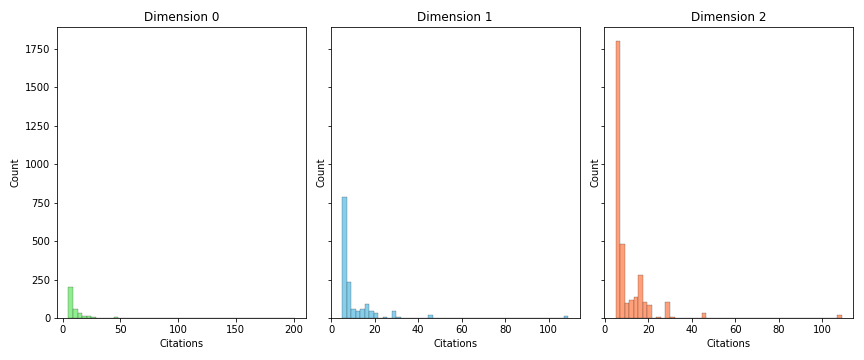
\includegraphics[scale=0.35]{./figures/distribution_cohain_150250.png}
% \caption{Distribution of the citation in CC1 } \label{fig:accuracy}
%\end{figure}
\begin{figure}[tb]
\centering
 \begin{subfigure}[t]{-0.8\textwidth}
 \vspace{-4cm}
    \text{(a)}
  \end{subfigure}
\begin{subfigure}[t]{0.8\textwidth}
\centering
   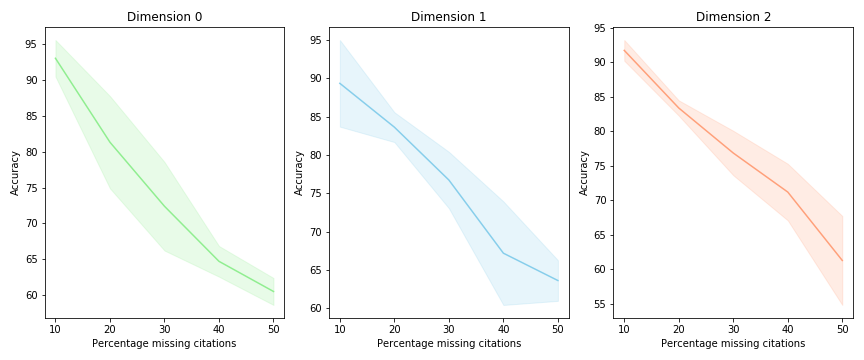
\includegraphics[scale=0.35]{./figures/accuracy_network1.png}
 %\caption{Accuracy of SNN in predicting missing citations } \label{fig:accuracy}
\end{subfigure}
 \begin{subfigure}[t]{0.8\textwidth}
    \text{(b)}
  \end{subfigure}
\begin{subfigure}[t]{0.8\textwidth}
\centering
\vspace{-0.5cm}
   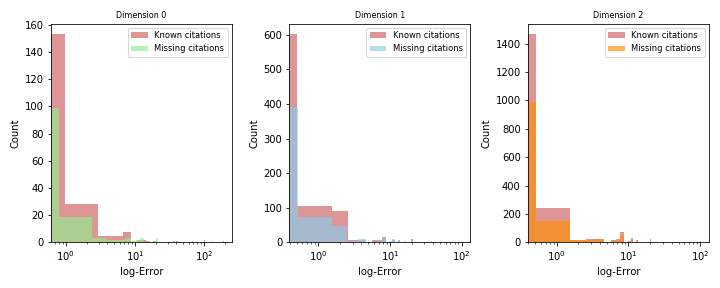
\includegraphics[scale=0.36]{./figures/Error_dist_start150250_seed6666_notsee40.png}
 % \caption{Distribution of the prediction's error} \label{fig:error}
\end{subfigure}
\caption{(a) Mean Accuracy $\pm$ std over 5 samples of SNN in imputing missing citations on CC1. (b)Mean Absolute Error $\pm$ std over 5 samples of SNN for $40\%$ missing values in CC1. \stefania{Add error on bins}}
\label{fig:accuracy-error}
\end{figure}
As a second assessment for our network we evaluate how accurately a SNN pretrained on a co-authorship complex can impute missing citations on a different complex. In Figure ~\ref{fig:transfer-learning} we show the MA in predicting missing citations on CC1 using the above architecture of SNN trained on CC2 (Co-authorship Complex 2, see Table~\ref{table:Simplices-coauthor}).
We compared our results with imputation methods based on statistical techniques, namely replacing missing data with the median or mean of the known data and inferring the missing values from the $(k-1)$ and $(k+1)$ neighbors of the simplices ($k$-simplicial neighbor $k$-sn). As Table~\ref{table:comparison-SNN} shows, SNNs outperform statistical techniques. Comparison with other state of the art imputations algorithms is left for future work.
\begin{figure}[htbp]
  \centering
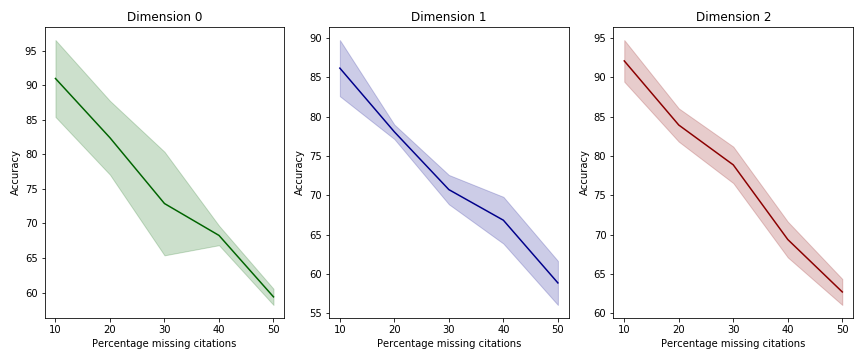
\includegraphics[scale=0.35]{./figures/accuracy_network1_pretrained.png}
  \caption{ Mean Accuracy $\pm$ std over 5 samples in imputing missing citations on CC1 of SNN trained on CC2 . } \label{fig:transfer-learning}
\end{figure}

%\scriptsize{
\begin{table}[htbp]
  \label{table:comparison-SNN}
  \centering
  \scriptsize{
  \begin{tabular}{c|cccccc}
    \cmidrule(r){1-7}
    Method   & CC1 - dim 0   & CC1 - dim 1   & CC1 - dim 2   & CC2 - dim 0  & CC2 - dim 1  & CC2 - dim 2 \\
    \midrule
    Mean & 1  & 12 & 1  & 1 & 1  & 1\\
    Median & 16 & 50 & 1  & 1& 1  & 1\\
    $k$-sn & 16 & 50& 1  & 1& 1  & 1 \\
    \bottomrule
  \end{tabular}}
  \caption


\section{Conlusion and Future Work}

FIXME

\begin{itemize}
\item Define pooling
\item Better baseline for the above work
\item Preliminary results on vector field data. Where we believe this method can be applied?
\item transfer learning accuracy is it linked to similar structure of complexes
\end{itemize}


\clearpage

\printbibliography

\end{document}
